\chapter{Crypto.Symmetric.AE}\label{AE}
Authenticated encryption (AE) schemes are symmetric-key mechanisms by
which a message M is transformed in to a ciphertext C in such a way
that C protects both privacy and authenticity
\cite{DBLP:journals/iacr/BellareRW03}. This package is specified in
\texttt{Crypto.Symmetric.AE}.
\subsubsection*{Generic Part}
\begin{lstlisting}{}
  generic
    type Key_Type is private;
    type Block is private;
    with package N is new Crypto.Types.Nonces(Block);
\end{lstlisting}
\subsubsection*{Types}
\begin{lstlisting}{}
  type AE_Scheme is limited interface;
  type Callback_Writer is access procedure (B : in  Bytes);
  type Callback_Reader is access procedure
  									(B : out Bytes; Count: out Natural);
\end{lstlisting}
In Ada \textbf{access} is like pointer in C++. Objects of an access
type, as the name implies, provide access to other objects and these
other objects can be allocated in a storage pool independent of the
block structure.

\subsubsection*{Procedures}
\begin{lstlisting}{}
  procedure Init_Encrypt(This   : out    AE_Scheme;
                         Key    : in     Key_Type;
                         Nonce  : in out N.Nonce'Class) is abstract;
  procedure Init_Decrypt(This        : out AE_Scheme;
                         Key         : in  Key_Type;
                         Nonce_Value : in  Block) is abstract;
  procedure Encrypt(This             : in out AE_Scheme;
                    Read_Plaintext   : in     Callback_Reader;
                    Write_Ciphertext : in     Callback_Writer) 
                    is abstract;
  function Decrypt_And_Verify
  					(This                   : in out AE_Scheme;
                Read_Ciphertext        : in Callback_Reader;
                Read_Ciphertext_Again  : in Callback_Reader := null;
                Write_Plaintext        : in Callback_Writer)
                return Boolean is abstract;
\end{lstlisting}
Notice that they are all abstract, they can not be called.

%%%%%%%%%%%%%%%%%%%%%%%%%%%%%%%%%%%%%%%%%%%%%%%%%%%%%%%%%%%%%%%%%%%%%
%%%%%%%%%%%%%%%%%%%%%%%%%%%%%%%%%%%%%%%%%%%%%%%%%%%%%%%%%%%%%%%%%%%%%

\section{AE.AD}
Authenticated Encryption with associated data (AEAD) is an extension
of the notion of authenticated encryption. The data has two fields, a
header ($H$) and a plaintext ($M$). The header $H$ consists of the
initial value/nonce $IV$. We denote an authenticated encryption scheme
with the requirement that the initial vector $IV$ is only used once in
a nonce based scheme. Otherwise, we call such a scheme deterministic
\cite{DBLP:conf/fse/FleischmannFL12}.
\subsubsection*{Types}
\begin{lstlisting}{}
  type AEAD_Scheme is limited interface;
\end{lstlisting}
\subsubsection*{Procedures}
\begin{lstlisting}{}
  procedure Encrypt(This            : in out AEAD_Scheme;
                    Read_Header     : in Callback_Reader;
                    Read_Plaintext  : in Callback_Reader;
                    Write_Ciphertext: in Callback_Writer)is abstract;
  function Decrypt_And_Verify
  				(This                   : in out AEAD_Scheme;
             Read_Header            : in     Callback_Reader;
             Read_Ciphertext        : in     Callback_Reader;
             Read_Ciphertext_Again  : in     Callback_Reader := null;
             Write_Plaintext        : in     Callback_Writer)
             return Boolean is abstract;
\end{lstlisting}
Notice that they are all abstract, they can not be called.\\

%%%%%%%%%%%%%%%%%%%%%%%%%%%%%%%%%%%%%%%%%%%%%%%%%%%%%%%%%%%%%%%%%%%%%
%%%%%%%%%%%%%%%%%%%%%%%%%%%%%%%%%%%%%%%%%%%%%%%%%%%%%%%%%%%%%%%%%%%%%

\section{AE\_OCB}
OCB stands for "Offset Codebook", which is fully parallelizable and
adds minor overhead. Desirable properties of OCB include the ability
to encrypt a string of arbitrary length, and no requirement for a
random IV \cite{DBLP:journals/tissec/RogawayBB03}. The OCB in the ACL
is defined as OCB3 by Ted Krovetz and Phillip Rogaway in
\cite{DBLP:conf/fse/KrovetzR11}. It shall be referred to as OCB
throughout this document.

\begin{figure}[h]
\centering
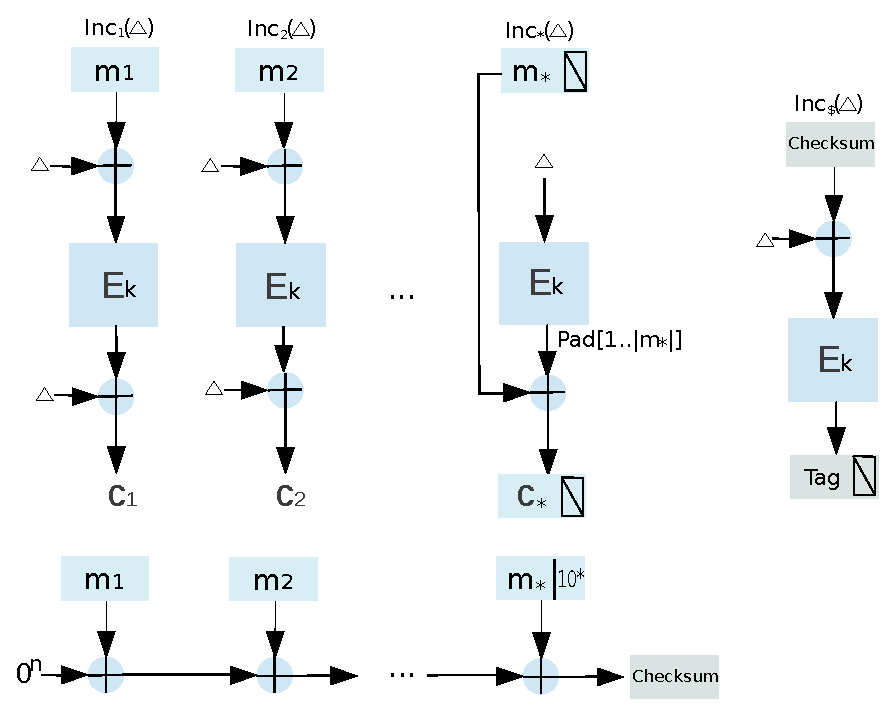
\includegraphics[scale=0.8]{./images/AE_OCB_En}
\caption{Workflow of the OCB encryption. Adapted from \cite{DBLP:conf/fse/KrovetzR11}.}\label{Workflow_OCB}
\end{figure}
Figure \ref{Workflow_OCB} shows the encryption of
AE\_OCB. \textbf{TOP} illustrates the situation of message M in a full
final block ($|M_4|=n$)(Checksum = $M_1\oplus M_2\oplus M_3\oplus
M_4$). \textbf{Bottom} is the situation that M has a short final
block, $1\leq |M_*|< n$,(Checksum = $M_1\oplus M_2\oplus M_3\oplus
M_*10^*$).

\subsubsection*{Generic Part}
\begin{lstlisting}{}
  generic
    with package BC is new Crypto.Symmetric.Blockcipher(<>);
    with package N is new Crypto.Types.Nonces(BC.Block);
    with function "xor" (Left, Right : in BC.Block)
    										return BC.Block is <>;
    with function To_Block_Type (B : Bytes) return BC.Block;
    with function To_Bytes (B : BC.Block) return Bytes;
    with function Shift_Left (Value: BC.Block; Amount: Natural)
    										return BC.Block;
    with function Shift_Right(Value: BC.Block; Amount: Natural)
    										return BC.Block;
    with function To_Byte_Word (X: Word) return Byte_Word;
\end{lstlisting}
The function \texttt{Shift\_Left()} is used to generate irreducible
polynomials $L(1..31)$. The function \texttt{Shift\_Right()} is used
to generate irreducible polynomial $L(-1)$.

\subsubsection*{Types}
\begin{lstlisting}{}
  type AE_OCB is new AE.AE_Scheme with private;
  Bytes_Per_Block : constant Positive := Block'Size / 8;
\end{lstlisting}
\subsubsection*{Procedures}
\begin{lstlisting}{}
  overriding
  procedure Init_Encrypt(This   : out    AE_OCB;
                         Key    : in     Key_Type;
                         Nonce  : in out N.Nonce'Class);
  overriding
  procedure Init_Decrypt(This        : out AE_OCB;
                         Key         : in  Key_Type;
                         Nonce_Value : in  Block);
  not overriding
  procedure Init_Encrypt(This             : out    AE_OCB;
                         Key              : in     Key_Type;
                         N_Init           : in out N.Nonce'Class;
                         Bytes_Of_N_Read  : in     Positive;
                         Taglen           : in     Positive);
  not overriding
  procedure Init_Decrypt(This             : out AE_OCB;
                         Key              : in  Key_Type;
                         N_Init           : in  Block;
                         Bytes_Of_N_Read  : in  Positive;
                         Taglen           : in  Positive);
\end{lstlisting}
The last two procedures with \textbf{not overriding} are additional
procedures. The overridden procedure \texttt{Init\_Encrypt()}
initializes private variables and prepares the key and $L$ array for
encryption. And the additional procedure \texttt{Init\_Encrypt()}
makes almost the same but with a user-defined tag length. In
overridden procedure \texttt{Init\_Decrypt()} all private variables
are initialized for decryption, and the additional procedure
\texttt{Init\_Decrypt()} makes initialization with a user-defined tag
length.\\

\noindent\textbf{Exception:} If the length of the nonce value in byte
(\texttt{Bytes\_Of\_N\_Read}) $>$ 16:
\texttt{Noncelength\-\_Not\_Supported}.

\hhline
\begin{lstlisting}{}
  overriding
  procedure Encrypt(This             : in out AE_OCB;
                    Read_Plaintext   : in     Callback_Reader;
                    Write_Ciphertext : in     Callback_Writer);
  overriding
  function Decrypt_And_Verify(This      : in out AE_OCB;
                 Read_Ciphertext        : in Callback_Reader;
                 Read_Ciphertext_Again  : in Callback_Reader := null;
                 Write_Plaintext        : in Callback_Writer)
                 return Boolean;
\end{lstlisting}
In encryption the plaintext is divided into blocks of fixed length, if
the final block is a short block, it will be padded with $10^*$. The
message will be processed block by block, and each time an
intermediate cipher block and a checksum (used to calculate tag later)
will be updated. A tag is produced during the last round. The final
output is then made of the ciphertext and the tag.\\

\noindent\textbf{Exception:}\\ The tag must be at least 1 byte, and
not greater than the block length,
otherwise:\\ \texttt{Invalid\_Ciphertext\_Error}\,.

%%%%%%%%%%%%%%%%%%%%%%%%%%%%%%%%%%%%%%%%%%%%%%%%%%%%%%%%%%%%
%%%%%%%%%%%%%%%%%%%%%%%%%%%%%%%%%%%%%%%%%%%%%%%%%%%%%%%%%%%%

\section{AEAD\_McOE}
McOE is a new family of on-line authenticated encryption (OAE)
schemes. An on-line manner means that the $i$-th ciphertext block can
be written before the ($i+1$)-th plaintext block has to be read
\cite{DBLP:conf/fse/FleischmannFL12}. Figure \ref{Mc} shows the
generic construction of McOE.
%\begin{figure}[htp]
%\centering
%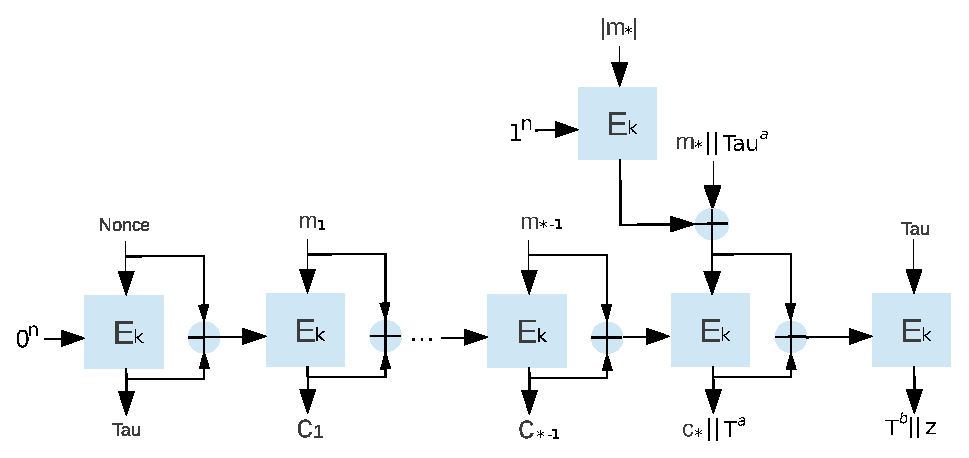
\includegraphics[scale=0.9]{./images/AE_McOE}
%\caption{The generic McOE workflow, where n is the block length,
  %Tau$^a$ denotes Tau[0..n-$|$m$_*|$-1], T$^a$ denotes a
  %(n-$|$c$_*|$)-bit string T[0..n-$|$c$_*|$-1] and T$^b$ denotes a
  %($|$c$_*|$)-bit string T[n-$|$c$_*|$..n]. T$^a$ and T$^b$ make up
  %the tag.  Adapted from
  %\cite{DBLP:conf/fse/FleischmannFL12}.}\label{Mc}
%\end{figure}

\subsubsection*{Generic Part}
\begin{lstlisting}{}
  generic
    type Block is private;
    type Key_Type is private;
    with package N is new Crypto.Types.Nonces(Block);
    with package Tweakable_Blockcipher is new
    	 	Crypto.Symmetric.Tweakable_Blockcipher(Block => Block, 
     					Key_Type   => Key_Type, Tweak_Type => Block);
    type TB_Type is new Tweakable_Blockcipher.TB_Interface 
    													with private;
    with function "xor"(Left,Right: Block) return Block is <>;
    with function To_Block_Type(B:in Bytes) return Block is <>;
    with function To_Byte_Word (X: Word) return Byte_Word; 
    with function To_Bytes(B : in Block) return Bytes;
\end{lstlisting}

\subsubsection*{Types}
\begin{lstlisting}{}
  type AEAD_McOE is new AE.AE_Scheme and AEAD.AEAD_Scheme
  with private;
\end{lstlisting}
When we compose interfaces in this way we can add new operations so
that the new interface such as \texttt{AEAD\_McOE} will have all the
operations of both \texttt{AE.AE\_Scheme} and \texttt{AEAD\_Scheme}
plus possibly some others declared specifically as operation of
\texttt{AEAD\_McOE}. \texttt{AE.AE\_Scheme} and
\texttt{AEAD.AEAD\_Scheme} are refered the progenitors of
\texttt{AEAD\_McOE}. The first one is not a parent, that term is only
used when deriving a type as opposed to composing an interface.

\subsubsection*{Procedures}
\begin{lstlisting}{}
 overriding
 procedure Encrypt(This             : in out AEAD_McOE;
                   Read_Plaintext   : in     Callback_Reader;
                   Write_Ciphertext : in     Callback_Writer);
 overriding
 procedure Encrypt(This             : in out AEAD_McOE;
                   Read_Header      : in     Callback_Reader;
                   Read_Plaintext   : in     Callback_Reader;
                   Write_Ciphertext : in     Callback_Writer);
 function Decrypt_And_Verify(This       : in out AEAD_McOE;
                   Read_Ciphertext      : in     Callback_Reader;
                   Read_Ciphertext_Again: in     Callback_Reader
                   													:= null;
                   Write_Plaintext      : in     Callback_Writer)
                               			return Boolean;
 function Decrypt_And_Verify(This       : in out AEAD_McOE;
                   Read_Header          : in     Callback_Reader;
                   Read_Ciphertext      : in     Callback_Reader;
                   Read_Ciphertext_Again: in     Callback_Reader 
                   													:= null;
                   Write_Plaintext      : in     Callback_Writer)
                               			return Boolean;
\end{lstlisting}
McOE uses a tweakable block cipher for encryption. Moreover, the
scheme specifies a so-called tag-split algorithm. In a normal
algorithm, the input will be padded if its length is smaller than the
block length, and the output is of a block length. The tag-split
algorithm is length-preserving, where the length of the output equals
the length of the input (before padding). The plaintext is divided
into blocks of fixed length $M=m_1m_2 \ldots m_{*}$. Full blocks are
encrypted without tag-split algorithm. For the case when the final
block is not full, the tag-splitting is applied. And the produced tag
is concatenated to the ciphertext.\\

\noindent\textbf{Exception:}\\ The appended tag is of a block length,
so a ciphertext has min. a block.  In the decryption of an invalid
ciphertext with the first block not
full:\quad\texttt{Invalid\_Ciphertext\_Error}.

%%%%%%%%%%%%%%%%%%%%%%%%%%%%%%%%%%%%%%%%%%%%%%%%%%%%%%%%%%%%%%%%%%%
%%%%%%%%%%%%%%%%%%%%%%%%%%%%%%%%%%%%%%%%%%%%%%%%%%%%%%%%%%%%%%%%%%

\section{AEAD\_SIV}
SIV is one of the five dedicated AE schemes. Rogaway and Schrimpton
proposed in their paper a provable key-wrapping algorithm (SIV -
Synthetic Initialization Vector Mode) that authenticates and encrypts
an arbitrary string and authenticates, but does not encryt, additional
data which can be bound into the wrapped key \cite{SIV}. The main
disadvantage is that they are inherently off-line: For encryption, one
must either keep the entire plaintext in memory, or read the plaintext
twice \cite{DBLP:conf/fse/FleischmannFL12}. Further details please
check RFC5297 \cite{SIV}. Figure \ref{SIVEN} shows the encryption
construction of SIV.
\begin{figure}[h]
\centering
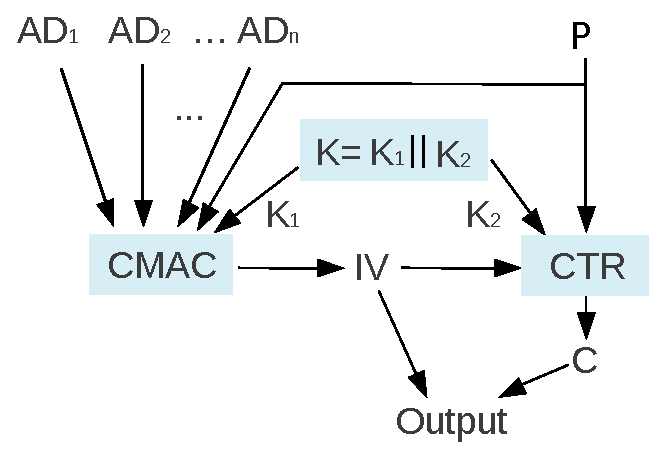
\includegraphics[scale=0.7]{./images/SIV_Encryption}
\caption{Workflow of the SIV encryption.}\label{SIVEN}
\end{figure}
The associated data is shown as $AD_1$ through $AD_n$, IV is the
synthetic IV, the ciphertext is C \cite{SIV}. The S2V process consists
the doubling and xoring operations on the output of CMAC. CTR is a
counter mode of AES.

\subsubsection*{Generic Part}
\begin{lstlisting}{}
  generic
    with package BC is new Crypto.Symmetric.Blockcipher(<>);
    with package N is new Crypto.Types.Nonces(BC.Block);
    with function "xor" (Left, Right : in BC.Block)
    										return BC.Block is <>;
    with function To_Block_Type (B : Bytes) return BC.Block;
    with function To_Bytes (B : BC.Block) return Bytes;
    with function Shift_Left (Value: BC.Block; Amount: Natural)
    										return BC.Block;
    with function "+" (Left: BC.Block; Right : in Byte)
    										return BC.Block is <>;
\end{lstlisting}

\subsubsection*{Types}
\begin{lstlisting}{}
 type AEAD_SIV is new AE.AE_Scheme and AEAD.AEAD_Scheme with private;
\end{lstlisting}

\subsubsection*{Procedures}
\begin{lstlisting}{}
  procedure Init_Enc(This   : out    AEAD_SIV;
                     Key1   : in     Key_Type;
                     Key2   : in     Key_Type);
  procedure Init_Dec(This   : out    AEAD_SIV;
                     Key1   : in     Key_Type;
                     Key2   : in     Key_Type);
  overriding
  procedure Encrypt(This             : in out AEAD_SIV;
                    Read_Plaintext   : in     Callback_Reader;
                    Write_Ciphertext : in     Callback_Writer);
  overriding
  procedure Encrypt(This             : in out AEAD_SIV;
                    Read_Header      : in     Callback_Reader;
                    Read_Plaintext   : in     Callback_Reader;
                    Write_Ciphertext : in     Callback_Writer);
  overriding
  function Decrypt_And_Verify(This      : in out AEAD_SIV;
                 Read_Ciphertext        : in Callback_Reader;
                 Read_Ciphertext_Again  : in Callback_Reader := null;
                 Write_Plaintext        : in Callback_Writer)
                     							return Boolean;
  overriding
  function Decrypt_And_Verify(This      : in out AEAD_SIV;
                 Read_Header            : in Callback_Reader;
                 Read_Ciphertext        : in Callback_Reader;
                 Read_Ciphertext_Again  : in Callback_Reader := null;
                 Write_Plaintext        : in Callback_Writer)
                               				return Boolean;
\end{lstlisting}
In preparation the key is set into two subkeys, which work in S2V and
CTR processes respectively. IV is used in CTR and also makes up the
final output as $IV||C$.

\subsubsection*{Example}
\begin{lstlisting}{}
  --Before calling the main program,
  --the interface functions should be implemented.
  procedure Example_SIV(T:in out Test_Cases.Test_Case'Class) is
    use AUnit.Assertions;
  begin
    SIV.Init_Enc(This => SIV_Type, Key1 => K1, Key2 => K2);
    SIV.Encrypt(This => SIV_Type, Read_Header => RH,
                Read_Plaintext => RP, Write_Ciphertext => WC);
    Put_Line("Ciphertext:");
    for I in 1..Natural(C_Vector.Length) loop
      Put(C_Vector.Element(I));
    end loop;
    C_Vector2 := C_Vector;
    Header_Index := 0;
    SIV.Init_Dec(This => SIV_Type, Key1 => K1, Key2 => K2);
    Verification_Bool := SIV.Decrypt_And_Verify
                      (This => SIV_Type, Read_Header => RH,
                       Read_Ciphertext => RC,
                       Read_Ciphertext_Again => RCA,
                       Write_Plaintext => WP);
    Put_Line(Verification_Bool'Img);
    if Verification_Bool then
      Put_Line("Plaintext:");
      for I in 1..Natural(Plain_Array.Length) loop
         Put(Plain_Array.Element(I));
      end loop;
    end if;
  end Example_SIV;
\end{lstlisting}
